% Converted from reference/DRSFlare (MadCap Flare, Java target)

\chapter{Replication With VOD}
\label{drs:db4o-replication-system-drs-vod-replication}

The Versant Object Database is the 'big brother' of db4o. It's an object database which can deal with a huge amount of data. Because it is also an object database it is a good partner for db4o. For scenarios where you have mobile devices which are synchronized against a big central datastore combining VOD and db4o makes sense. db4o for the mobile end device and VOD on the central server. The Java version of dRS supports therefore this replication between db4o and VOD.

\textbf{Note: Replication with VOD requires at least VOD version 8.0.1.3 with JVI installed.}

The VOD replication partner has to be prepared to be ready for replication. The replication is based on the JDO-interface. Therefore you need to setup and use JDO for the replication. \hyperref[drs:db4o-replication-system-drs-vod-setup]{See "Setup JDO for VOD"} (p.~\pageref{drs:db4o-replication-system-drs-vod-setup})

Additionally a special event processor has to be installed which is responsible to keep track of changes for upcoming replications. \hyperref[drs:db4o-replication-system-drs-vod-setup-event-processing]{See "Setup Event Processing"} (p.~\pageref{drs:db4o-replication-system-drs-vod-setup-event-processing})

After everything is up and running you can start to replicate between db4o and VOD. \hyperref[drs:db4o-replication-system-drs-vod-vod-replication]{See "VOD Replication"} (p.~\pageref{drs:db4o-replication-system-drs-vod-vod-replication})

\section{Setup JDO for VOD}
\label{drs:db4o-replication-system-drs-vod-setup}

This guide shows how to setup JDO for VOD.

This topic assumes that you've already installed the VOD database. VOD is a separate, commercial product, now sold by Actian; follow its installation guide.

\subsection{Create A Database}
\label{drs:db4o-replication-system-drs-vod-setup:createdb}

The first step is to create the database. If you already have a database you can skip this step. The official documentation on managing the VOD database can be found in the VOD installation-folder.

You can create the database with the 'Administration Console' which is shipped with VOD. Start the 'Administration Console', choose 'File'-\textgreater{}'Create Database...' and follow the wizard to create a new database.

As alternative you can create a new database in the command line with these commands:

\begin{lstlisting}
makedb databaseName@localhost
createdb databaseName@localhost
startdb databaseName@localhost
\end{lstlisting}

\subsection{JDO Setup}
\label{drs:db4o-replication-system-drs-vod-setup:jdosetup}

The replication system uses the JDO API to replicate objects between db4o and VOD. Therefore you need to setup the VOD JDO implementation. Again the official documentation is part of the VOD installation. This is just a very short guide to setting JDO up and doesn't cover all details.

First you need to add the JDO-libraries to you project. The JDO-libraries are in the VOD-directory under the 'lib'-subdirectory. You need to add at least these jars.

\begin{itemize}
\item jdo2-api-2.1.jar
\item vodjdo.jar
\item asm-all-3.1.jar
\item jta-1.1.jar
\end{itemize}

Second you need to provide the JDO configuration. You can keep this information in a property file. For example in a versant.properties-file which is stored along with your code. There are three important configuration settings you need to set, the factory-class, the connection-URL and information which classes are enhanced.

For more properties and settings read the JDO and VOD documentation. The example property-file looks like this:

\begin{lstlisting}
## The implementation of the JDO standard
javax.jdo.PersistenceManagerFactoryClass=com.versant.core.jdo.BootstrapPMF
# The connection-string
javax.jdo.option.ConnectionURL=versant:dRSVodExample
# Files which contain a list of meta information for the persistent
# classes. You can list more with versant.metadata.1= versant.metadata.2= ... versant.metadata.n
versant.metadata.0=com/db4odoc/drs/vod/package.jdo
\end{lstlisting}

{\small\itshape versant.properties: JDO configuration for VOD\par}
\medskip

Additionally you need to have a package description where you declare all persistent classes:

\begin{lstlisting}
<jdo>
    <package name="com.db4odoc.drs.vod">
        <class name="com.db4odoc.drs.vod.Car"/>
        <class name="com.db4odoc.drs.vod.Pilot"/>
    </package>
</jdo>
\end{lstlisting}

{\small\itshape package.jdo: List all persistent classes of this package\par}
\medskip

The last preparation step is to get the enhancer in place. JDO requires that classes implements the PersistenceCapable interface. Implementing this by hand would be extremely painful. That's why you can use an enhancer which does this for you. Create an Ant build script which does that.

\begin{lstlisting}
<project name="tutorial" default="build-and-enhance" basedir=".">

    <property file="machine.properties"/>
    <!--The location of the build-result (the compiled class-files).
     Depends on you're build-system / IDE.
     For plain Eclipse projects it's usually "./bin" -->
    <property name="dir.build.output" value="./bin"/>
    <property name="dir.build.source" value="./src"/>
    <property name="dir.lib" value="./lib"/>

    <property name="dir.jdo.lib" value="${dir.vod.install.location}\lib"/>
    <property name="dir.jdo.sdklib" value="${dir.vod.install.location}\sdk\lib"/>

    <path id="enhancerClassPath">
        <pathelement  path="${dir.build.output}"/>
        <fileset dir="${dir.jdo.lib}" includes="**/*.jar"/>
        <fileset dir="${dir.jdo.sdklib}" includes="**/*.jar"/>
    </path>

    <target name="build-and-enhance" depends="compile, enhance"/>

    <target name="enhance" description="Enhance the JOD classes">
        <taskdef resource="versant.tasks">
            <classpath>
                <path refid="enhancerClassPath"/>
            </classpath>
        </taskdef>

        <jdo-enhance outputdir="${dir.build.output}"
                     classpathref="enhancerClassPath" >
            <persistentaware dir="${dir.build.output}"/>
        </jdo-enhance>
    </target>

    <target name="compile">
        <mkdir dir="${dir.build.output}"  />
        <javac srcdir="${dir.build.source}"
            destdir="${dir.build.output}"
            target="6"
            source="6"
            debug="on"
            encoding="UTF-8">
                <classpath>
                    <pathelement path="${dir.jdo.lib}/jdo2-api-2.1.jar"/>
                    <pathelement path="${dir.jdo.lib}/vodjdo.jar"/>
                    <pathelement path="${dir.jdo.lib}/asm-all-3.1.jar"/>
                    <pathelement path="${dir.lib}/*"/>
                </classpath>
            </javac>
        <copy todir="${dir.build.output}">
            <fileset dir="${dir.build.source}" casesensitive="yes">
              <include name="**/*.*"/>
              <exclude name="**/*.java"/>
            </fileset>
        </copy>
    </target>
</project>
\end{lstlisting}

{\small\itshape build.xml: Enhancer script\par}
\medskip

Along to the Ant-script add a machine.properties-file, which contains the installation specific information. Like the installation-location of VOD.

\begin{lstlisting}
# The installation folder of VOD
dir.vod.install.location=C:/progs/Versant/8
\end{lstlisting}

{\small\itshape machine.properties: The properties for our project\par}
\medskip

\subsection{Using JDO}
\label{drs:db4o-replication-system-drs-vod-setup:usingjdo}

After running the enhancer you can start using JDO. First you need to create a PersistenceManagerFactory-instance. This can be created with the static helper methods from the JDOHelper-class:

\begin{lstlisting}
InputStream propertySource = Thread.currentThread()
        .getContextClassLoader().getResourceAsStream(VERSANT_PROPERTY_FILE);
if (null == propertySource) {
    throw new RuntimeException("Couldn't find resource '" + VERSANT_PROPERTY_FILE + "' in the classpath");
}
try {
    return JDOHelper.getPersistenceManagerFactory(propertySource);
} finally {
    try {
        propertySource.close();
    } catch (IOException ignored) {
    }
}
\end{lstlisting}

{\small\itshape JDOUtilities.java: Opening the persistence factory\par}
\medskip

After that you can create persistence manager with the factory and use it to store, query and update objects with JDO:

\begin{lstlisting}
PersistenceManagerFactory factory = JDOUtilities.createPersistenceFactory();

PersistenceManager persistence = factory.getPersistenceManager();
persistence.currentTransaction().begin();

Pilot john = new Pilot("John",42);
Car car = new Car(john,"Fiat Punto");

persistence.makePersistent(car);

persistence.currentTransaction().commit();
persistence.close();
\end{lstlisting}

{\small\itshape StoreObjectsWithJDO.java: Use the persistence manager to store objects\par}
\medskip

For more information and help on JDO read the official VOD documentation and take a look the \href{https://www.datanucleus.org/products/accessplatform/jdo/}{JOD API}.

\section{Setup Event Processing}
\label{drs:db4o-replication-system-drs-vod-setup-event-processing}

The replication system needs to know which objects have been changed in order to replicate these changes. To do so it uses VOD's event system. You need to setup the event processing and keep it running for this purpose.

\textbf{Note: Replication with VOD requires at least VOD version 8.0.1.3 with JVI installed.}

\subsection*{The Classpath}

For the replication operations some additional libraries are required besides the JDO ones. This includes the db4o related libraries and additional VOD libraries.

From the VOD distribution

\begin{itemize}
\item jdo2-api-2.1.jar
\item vodjdo.jar
\item asm-all-3.1.jar
\item antlr-3.1.1-runtime.jar
\item jta-1.1.jar
\item jvi80.jar
\end{itemize}

From db4o / dRS

\begin{itemize}
\item db4o-8.1-core.jar (or db4o-8.1-all.jar)
\item dRS-8.1-core.jar
\end{itemize}

\begin{itemize}
\item commons-cli-1.2.jar
\end{itemize}

\subsection{Creating the Event Schema}
\label{drs:db4o-replication-system-drs-vod-setup-event-processing:eventschema}

The event processing needs special schema's to work correctly. Therefore you need to setup the event schema. You can do this by running the CreateEventSchema-class which does this for you. Pass the database name as argument to that class. You can execute this from the command line, where the classpath contains the libraries from above.

Windows:

\begin{lstlisting}
java -classpath %CLASSPATH% com.db4o.drs.versant.eventprocessor.CreateEventSchema %DATABASE_NAME%
\end{lstlisting}

Unix/Linux:

\begin{lstlisting}
java -classpath $CLASSPATH com.db4o.drs.versant.eventprocessor.CreateEventSchema $DATABASE_NAME
\end{lstlisting}

\subsection{Running The Event Driver}
\label{drs:db4o-replication-system-drs-vod-setup-event-processing:eventdriver}

The next step is to run the VOD event driver. The event driver is a small service application for processing database events. You need to keep the event driver running all the time when you're using replication. Without a running event driver modifications are not replicated. You need to create a configuration file for the event driver.

Windows config.ved.win:

\begin{lstlisting}
ChannelServicePort    4000
LogFile eventdb.log
LogLevel 2
<EngineLibs>
vedse.dll
</EngineLibs>
\end{lstlisting}

Unix/Linux config.ved.linux:

\begin{lstlisting}
ChannelServicePort    4000
LogFile eventdb.log
LogLevel 2
<EngineLibs>
libvedse.so
</EngineLibs>
\end{lstlisting}

With this configuration you can run the event driver. Execute the veddriver command where the first argument is the database name and the second argument is the configuration-file:

\begin{lstlisting}
veddriver %DATABASE_NAME% %VED_CONFIGFILE%
\end{lstlisting}

When veddriver executable is in the 'bin'-subdirectory of your VOD installation.

\subsection{Running The Event Processor}
\label{drs:db4o-replication-system-drs-vod-setup-event-processing:eventprocessor}

After the event driver is up and running we finally can start to process the events. This event processing is there to maintain additional meta-information for the replication process. Ensure that the event processor it always up and running. If it isn't running changes are not replicated.

The event processor is part of the db4o replication system. It's in the EventProcessorApplication-class. This class needs these parameters:

{\small
\begin{longtable}{|p{\dimexpr(\linewidth-4\arrayrulewidth)*1/3-2\tabcolsep\relax}|p{\dimexpr(\linewidth-4\arrayrulewidth)*1/3-2\tabcolsep\relax}|p{\dimexpr(\linewidth-4\arrayrulewidth)*1/3-2\tabcolsep\relax}|}
\hline
-database &  & The name of the database which is replicated \\ \hline
-server & Optional & The host name of the machine where the VOD event driver is running.This a optional parameter. If it's not specified it assumes that the event driver is running on the localhost. \\ \hline
-servertport &  & The port of the VOD event driver. It's the port specified in the event driver configuration. In this example it's 4000 \\ \hline
-client & Optional & The VOD event driver contacts the event processor on certain events. With this parameter you specify the host-name on which the event processor runs. It this parameter is not set localhost will be used. \\ \hline
-clientport &  & The port which is used for the client. It can be any free port. \\ \hline
-eventProcessorPort &  & The port on which the event processor listens for replication processes. The replication process connects to this port. \\ \hline
-logfile &  & Specifies the log file. \\ \hline
-verbose & Optional & Enable the verbose messages \\ \hline
\end{longtable}}

To start the event processor you can use this command. Use the classpath-variable refers to the classpath listed above.

Windows:

\begin{lstlisting}
java -cp %CLASSPATH% com.db4o.drs.versant.eventprocessor.EventProcessorApplication -clientport 4100 -database %DATABASE_NAME% -eventProcessorPort 4088 -logfile %LOG_FILE% -serverport 4000
\end{lstlisting}

Linux:

\begin{lstlisting}
java -cp $CLASSPATH com.db4o.drs.versant.eventprocessor.EventProcessorApplication -clientport 4100 -database $DATABASE_NAME -eventProcessorPort 4088 -logfile $LOG_FILE  -serverport 4000
\end{lstlisting}

\subsection{Example Scripts}
\label{drs:db4o-replication-system-drs-vod-setup-event-processing:examplescripts}

You can use scripts to do this tasks described above. .

You need to adopt the setEnviroment-script to you environment. Specify the path where dRS and db4o jars are. Additionally it expects that the JAVA\_HOME and the VERSANT\_ROOT environment variables are set. The JAVA\_HOME should point to your java-installation. The VERSANT\_ROOT should point to the VOD installation directory.

Windows:

\begin{lstlisting}
REM Specify the directory where the DRS and db4o jars are
REM This directory should contain the db4o and dRS jars.
REM Or more specific it needs the dRS-8.1-core.jar, 
REM db4o-8.1-core.jar or db4o-8.1-core.jar, commons-cli-1.2.jar
SET LIB_DIR=./lib

REM Specify the VOD database name
SET DATABASE_NAME=dRSVodExample

REM Set the directory where VOD is installed. For example "C:\Program Files\Versant\8"
SET VERSANT_ROOT=%VERSANT_ROOT%

REM This should work if the JAVA_HOME variable is set. 
REM Otherwise change the command to point to the java executatble or set the JAVA_HOME variable
SET JAVA=java
JAVA_HOME=$JAVA_HOME
\end{lstlisting}

{\small\itshape setEnvironment.bat: The imporatent configuration items\par}
\medskip

Linux:

\begin{lstlisting}
# Specify the directory where the DRS and db4o jars are
# This directory should contain the db4o and dRS jars.
# Or more specific it needs the dRS-8.1-core.jar, 
# db4o-8.1-core.jar or db4o-8.1-core.jar, commons-cli-1.2.jar
LIB_DIR=./lib

# Specify the VOD database name
DATABASE_NAME=dRSVodExample

# Set the directory where VOD is installed. For example "C:\Program Files\Versant\8"
VERSANT_ROOT=$VERSANT_ROOT

# This should work if the JAVA_HOME variable is set. 
# Otherwise change the command to point to the java executatble or set the JAVA_HOME variable
JAVA=java.exe
JAVA_HOME=$JAVA_HOME
\end{lstlisting}

{\small\itshape setEnvironment.sh: The imporatent configuration items\par}
\medskip

After that you can use the provided scripts to do the steps above.

\begin{itemize}
\item createDatabase: This scripts creates a database with the name configured in DATABASE\_NAME
\item createEventSchema: This script creates the schema for the event processing
\item startEventDriver: This script starts the event driver
\item startEventProcessor: This script starts the event processor
\end{itemize}

\subsection*{Start the Event Driver and Event Processor With Your Database}

In a production environment the event driver and event processor have to run all the time. Therefore it makes sense to start up these two processes together with your database.

You can do this by adding startup entries to your database configuration.

First copy the scripts for starting the event processor to your VOD database directory. Edit the script so that it works from the new location. In the example scripts you probably have to change the directory where the libraries reside.

Second add two new configuration entries to the profile.be file:

\begin{lstlisting}
event_daemon veddriver  the/path/to/config.ved.win
startup_script startEventProcessor.bat
\end{lstlisting}

Then restart the database. These configuration entries should ensure that the event driver and processor are started together with the VOD database.

\section{VOD Replication}
\label{drs:db4o-replication-system-drs-vod-vod-replication}

After setting up \hyperref[drs:db4o-replication-system-drs-vod-setup]{JDO} (p.~\pageref{drs:db4o-replication-system-drs-vod-setup}) and the \hyperref[drs:db4o-replication-system-drs-vod-setup-event-processing]{event processing} (p.~\pageref{drs:db4o-replication-system-drs-vod-setup-event-processing}) we're ready to start the replication.

\textbf{Note: Replication with VOD requires at least VOD version 8.0.1.3 with JVI installed.}

\subsection*{Classpath}

For the VOD replication following libraries need to be in the class-path:

From the VOD distribution

\begin{itemize}
\item jdo2-api-2.1.jar
\item vodjdo.jar
\item asm-all-3.1.jar
\item antlr-3.1.1-runtime.jar
\item jta-1.1.jar
\item jvi80.jar
\end{itemize}

From db4o / dRS

\begin{itemize}
\item db4o-8.1-core.jar (or db4o-8.1-all.jar)
\item dRS-8.1-core.jar
\end{itemize}

\subsection{Prepare db4o}
\label{drs:db4o-replication-system-drs-vod-vod-replication:prepare}

The first thing you need to do is preparing db4o for replication. Enable the UUID and version-number support for your database. UUID's are used to recognize objects across the database boundary. The version number is used the track changes.

Because classes are enhanced for JDO they have additional fields. To avoid that these artificial fields are stored in the db4o database you need to use the JDOReflector. This reflector recognized JDO -aware objects and treats them differently.

\begin{lstlisting}
EmbeddedConfiguration config = Db4oEmbedded.newConfiguration();
config.file().generateUUIDs(ConfigScope.GLOBALLY);
config.file().generateCommitTimestamps(true);
config.common().reflectWith(
        new JdoReflector(Thread.currentThread().getContextClassLoader()));
\end{lstlisting}

{\small\itshape SimpleReplication.java: Enable UUIDs and commit timestamps use the JDO reflector\par}
\medskip

\subsection{Replication From db4o To VOD}
\label{drs:db4o-replication-system-drs-vod-vod-replication:db4otovod}

After this preparation you can store, retrieve and update normally. To start the replication-process you need to create the two replication partners. Open a replication partner for db4o like this:

\begin{lstlisting}
ReplicationProvider mobileDatabase
        = new Db4oEmbeddedReplicationProvider(container);
\end{lstlisting}

{\small\itshape SimpleReplication.java: Open the db4o replication provider\par}
\medskip

Then open a replication provider for VOD. First create a new VodDatabase instance by passing the JDO PersistenceManagerFactory or the \hyperref[drs:db4o-replication-system-drs-vod-setup]{configuration properties} (p.~\pageref{drs:db4o-replication-system-drs-vod-setup}) to the constructor.

Second configure the host and port of the event processor with the configureEventProcessor method. Use the port which you've configured when setting up the \hyperref[drs:db4o-replication-system-drs-vod-setup-event-processing]{event processor} (p.~\pageref{drs:db4o-replication-system-drs-vod-setup-event-processing}). It's the port you've configured with the '-eventProcessorPort'-configuration.

Then create the VOD replication provider. For the VOD replication provider you should additionally add all classes which you want to replicate. Why is this necessary? In VOD you usually have a huge database and you only want to replicate parts of it to db4o. Therefore you can specify which classes are replicated. In case you don't specify anything only the types which have been already replicate once are replicated.

\begin{lstlisting}
VodDatabase vodDatabase = new VodDatabase(factory);
vodDatabase.configureEventProcessor("localhost",4088);
VodReplicationProvider centralDatabase
        = new VodReplicationProvider(vodDatabase);
centralDatabase.listenForReplicationEvents(Car.class, Pilot.class);
\end{lstlisting}

{\small\itshape SimpleReplication.java: Open the VOD replication provider\par}
\medskip

After that you can start the replication. Request the changes from the db4o replication provider. Then iterate over the changed objects and replicate them. Commit to complete the replication process.

\begin{lstlisting}
ReplicationSession replicationSession =
        Replication.begin(mobileDatabase, centralDatabase);

ObjectSet changesOnMobileDB = mobileDatabase.objectsChangedSinceLastReplication();
for (Object changedObject : changesOnMobileDB) {
    replicationSession.replicate(changedObject);
}
replicationSession.commit();
\end{lstlisting}

{\small\itshape SimpleReplication.java: Start replication\par}
\medskip

After this we've replicated the objects from db4o to VOD.

\subsection{Replicate From VOD To db4o}
\label{drs:db4o-replication-system-drs-vod-vod-replication:vodtodb4o}

To replicate from VOD to db4o ensure that you have configured the VOD replication provider properly. You need to add the types which you're going to replicate.

\begin{lstlisting}
VodDatabase vodDatabase = new VodDatabase(factory);
vodDatabase.configureEventProcessor("localhost",4088);
VodReplicationProvider centralDatabase
        = new VodReplicationProvider(vodDatabase);
centralDatabase.listenForReplicationEvents(Car.class, Pilot.class);
\end{lstlisting}

{\small\itshape SimpleReplication.java: Open the VOD replication provider\par}
\medskip

To replicate from VOD to db4o you just need to change the replication direction. Take the changes from the VOD database and replicate them to db4o.

\begin{lstlisting}
ReplicationSession replicationSession =
        Replication.begin(mobileDatabase, centralDatabase);

ObjectSet changesOnVOD = centralDatabase.objectsChangedSinceLastReplication();
for (Object changedObject : changesOnVOD) {
    replicationSession.replicate(changedObject);
}
replicationSession.commit();
\end{lstlisting}

{\small\itshape SimpleReplication.java: From VOD to db4o\par}
\medskip

\subsection{Bidirectional Replication}
\label{drs:db4o-replication-system-drs-vod-vod-replication:bidirectional}

To replicate bidirectional you need to get the changes from both databases and then replicate those changes.

\begin{lstlisting}
ReplicationSession replicationSession =
        Replication.begin(mobileDatabase, centralDatabase);

ObjectSet changesOnDB4O = mobileDatabase.objectsChangedSinceLastReplication();
for (Object changedObject : changesOnDB4O) {
    replicationSession.replicate(changedObject);
}

ObjectSet changesOnVOD = centralDatabase.objectsChangedSinceLastReplication();
for (Object changedObject : changesOnVOD) {
    replicationSession.replicate(changedObject);
}
replicationSession.commit();
\end{lstlisting}

{\small\itshape SimpleReplication.java: Bidirectional replication\par}
\medskip

\section{Replicating to a Mobile Device}
\label{drs:db4o-replication-system-drs-vod-replicating-to-mobile-device}

To replicate against VOD you need all the dependencies for VOD which also includes some native libraries. How can you avoid these extra dependencies?

\subsection{The Workaround}
\label{drs:db4o-replication-system-drs-vod-replicating-to-mobile-device:workaround}

Currently there is one work-around. You can start up a db4o server, which acts an intermediate replication server. The clients replicate against that db4o server and the server then replicates to the VOD server. These are the steps which you need to do:

\begin{enumerate}
\item Setup a db4o server.
\item Setup a periodic replication between the db4o server and VOD.
\item Create the clients, which replicate against the db4o server.
\end{enumerate}

\begin{center}
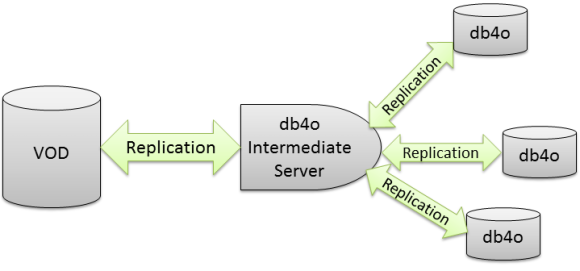
\includegraphics[width=\maxwidth]{images/drs-db4o-replication-system-drs-vod-mobile-replication.png}
\end{center}
\subsection{Setup the Intermediate db4o Server}
\label{drs:db4o-replication-system-drs-vod-replicating-to-mobile-device:intermediate}

The intermediate db4o server will act as replication server. It needs following dependencies:

From the VOD distribution

\begin{itemize}
\item jdo2-api-2.1.jar
\item vodjdo.jar
\item asm-all-3.1.jar
\item antlr-3.1.1-runtime.jar
\item jta-1.1.jar
\item jvi80.jar
\end{itemize}

From db4o / dRS

\begin{itemize}
\item db4o-8.1-core.jar (or db4o-8.1-all.jar)
\item dRS-8.1-core.jar
\end{itemize}

\begin{itemize}
\item db4o-8.1-cs.jar (not needed when you use the db4o-8.1-all.jar)
\end{itemize}

After that you can start a db4o server. Note that it is a pure in memory server, since it does not act a persistent store. For more details take a look at the db4o reference documentation.

\begin{lstlisting}
ServerConfiguration config = Db4oClientServer.newServerConfiguration();
config.file().generateUUIDs(ConfigScope.GLOBALLY);
config.file().generateCommitTimestamps(true);
config.file().storage(new PagingMemoryStorage());
config.common().reflectWith(new JdoReflector(Thread.currentThread().getContextClassLoader()));
ObjectServer server = Db4oClientServer.openServer(config, "!In:Memory!", 8080);
server.grantAccess("sa", "sa");
\end{lstlisting}

{\small\itshape IntermediateDb4oServer.java: Setup server\par}
\medskip

\subsection{Setup Periodic Replication}
\label{drs:db4o-replication-system-drs-vod-replicating-to-mobile-device:periodic}

The next step is to setup periodic replication between the VOD server and the db4o server. Take a look at how to replicate \hyperref[drs:db4o-replication-system-drs-vod-vod-replication]{against VOD here} (p.~\pageref{drs:db4o-replication-system-drs-vod-vod-replication}). The only difference is that it is executed periodically against the intermediate db4o server.

\begin{lstlisting}
final Timer timer = new Timer(true);
timer.schedule(new TimerTask() {
            @Override
            public void run() {
                runReplication();
            }
        },0, TEN_SECONDS_IN_MILLISEC);
\end{lstlisting}

{\small\itshape IntermediateDb4oServer.java: Schedule every 10 seconds\par}
\medskip

The replication against VOD is the same \hyperref[drs:db4o-replication-system-drs-vod-vod-replication]{like here} (p.~\pageref{drs:db4o-replication-system-drs-vod-vod-replication}), but with a db4o client.

\begin{lstlisting}
private void runReplication() {
    ClientConfiguration config = Db4oClientServer.newClientConfiguration();
    config.common().reflectWith(new JdoReflector(Thread.currentThread().getContextClassLoader()));
    ObjectContainer intermediate = Db4oClientServer.openClient(config,"localhost",8080,"sa","sa");
        ReplicationProvider mobileDatabase
            = new Db4oClientServerReplicationProvider(intermediate);
    // The rest is just the regular replication stuff
\end{lstlisting}

{\small\itshape IntermediateDb4oServer.java: Replicate with the db4o server\par}
\medskip

\subsection{The Client}
\label{drs:db4o-replication-system-drs-vod-replicating-to-mobile-device:client}

Now the client doesn't need any VOD dependencies, since we replicate via a db4o server. It needs these dependencies:

\begin{itemize}
\item db4o-8.1-core.jar (or db4o-8.1-all.jar)
\item dRS-8.1-core.jar
\item db4o-8.1-cs.jar (not needed when you use the db4o-8.1-all.jar)
\end{itemize}

Additionally the client needs the classes of the stored objects, but the not enhanced version of the classes. So you have to make sure that you've the original classes on the client and the enhanced classes on the server.

After that the replication is very easy. You just connect to the db4o server and replicate the objects. \hyperref[drs:db4o-replication-system-drs-db4o-databases-replication-bi-directional-replication]{See "Bidirectional Replication"} (p.~\pageref{drs:db4o-replication-system-drs-db4o-databases-replication-bi-directional-replication})

\begin{lstlisting}
EmbeddedConfiguration config = Db4oEmbedded.newConfiguration();
config.file().generateUUIDs(ConfigScope.GLOBALLY);
config.file().generateCommitTimestamps(true);
ObjectContainer theMobileDatabase = Db4oEmbedded.openFile(config, "mobileDatabase.db4o");
ObjectContainer db4oServer = Db4oClientServer.openClient("localhost", 8080, "sa", "sa");
try {
    ReplicationProvider localProvider = new Db4oEmbeddedReplicationProvider(theMobileDatabase);
    ReplicationProvider remoteProvider = new Db4oClientServerReplicationProvider(db4oServer);

    final ReplicationSession replicationSession = Replication.begin(localProvider, remoteProvider);

    replicateAll(replicationSession,localProvider.objectsChangedSinceLastReplication());
    replicateAll(replicationSession,remoteProvider.objectsChangedSinceLastReplication());

    replicationSession.commit();

} catch (Exception e){
    throw new RuntimeException(e);
} finally{
    db4oServer.close();
    theMobileDatabase.close();
}
\end{lstlisting}

{\small\itshape ClientReplicator.java: Replicate against the db4o intermediate server\par}
\medskip

